%------------------------------------------------------------
% Experimentos e resultados
%------------------------------------------------------------

\chapter{Experimentos e Resultados}
\label{experimentos}

Os experimentos realizados nesta pesquisa evoluem mapas para um jogo de aventura utilizando os métodos e funções previamente elaborados nos capítulos anteriores. O objetivo dos experimentos é testar e comprovar a eficiência do método proposto em obter mapas diversificados e com boas notas de avaliação em comparação à outras técnicas.

Quatro configurações de execuções foram consideradas para os testes: \textbf{algoritmo genético (AG)}, \textbf{busca inovativa (NS)}, \textbf{busca inovativa com competição local (Lehman)} e \textbf{busca inovativa com competição local e critério mínimo (Proposta)}.

A primeira configuração utiliza somente a função de avaliação definida para evoluir os mapas da forma tradicional de um algoritmo genético. Esta configuração é utilizada como controle para obtenção de dados base e comparação das notas de avaliação obtidas por outros métodos.

A segunda configuração é a implementação direta da NS, utilizando somente a função de distância definida para a evolução da população. Esta é outra configuração de controle que tem a finalidade de demonstrar que sem uma pressão para adaptação em prol da função de avaliação, os indivíduos gerados, embora bem diversificados, tendem a ter uma nota de avaliação baixa.

A terceira configuração é baseada na implementação proposta em \cite{lehman2011evolving}, que utiliza um MOEA (NSGA-II) para combinar a função de dispersão com a função de avaliação local. Desta forma a competição é restringida aos indivíduos próximos em relação ao espaço gerado pela função de dispersão, onde cada indivíduo é recompensado em relação ao número de vezes que sua nota de avaliação é superior à nota de seus vizinhos.

A configuração final é uma modificação proposta para a terceira configuração com a inclusão da ideia de critério mínimo. Nesta configuração, assim como na terceira, utiliza-se um MOEA (NSGA-II) para combinar a função de dispersão com a função de avaliação local, mas ao invés de utilizar a NS para evoluir a população, ela utiliza uma versão modificada da PMCNS, onde indivíduos que não atingem um critério mínimo, baseado em sua nota de avaliação, recebem uma nota de avaliação local igual a zero. Desta forma indivíduos funcionalmente muito inferiores possuem menores chances durante a seleção, mas ainda podem ser selecionados caso tenham altas notas em relação à função de dispersão, continuando a contribuir com o aumento da diversidade fenotípica.

\section{Parâmetros de Execução}

O tamanho da população em todos os experimentos é de 200 indivíduos, e uma execução corresponde à 200 gerações. A taxa de troca genética foi configurada à 75\% e a taxa de mutação à 5\% para todas as configurações. As configurações \textbf{AG} e \textbf{NS} utilizam a seleção elitista com base na função de avaliação e função de dispersão respectivamente, enquanto a seleção nas configurações \textbf{Lehman} e \textbf{Proposta} são baseadas na seleção utilizada pelo NSGA-II (também elitista) com base na função de dispersão e nota de avaliação local. Em ambos os casos, o NSGA-II utiliza a ordenação por dispersão dentro de cada frente não-ordenada, conforme apresentado previamente.

Enquanto a configuração \textbf{AG} é baseada em um algoritmo genético clássico, as configurações \textbf{NS}, \textbf{Lehman} e \textbf{Proposta} utilizam a PMCNS para evoluir suas populações. Nas configurações \textbf{NS} e \textbf{Lehman} os parâmetros de critério mínimo inicial (${cm}_0$), exigência do critério mínimo ($P$) e fator de suavização ($S$) são todos iguais a 0 para obter os mesmos resultados da NS comum; na configuração \textbf{Proposta} temos ${cm}_0=0$, $P=0.5$ e $S=0.5$ realizando efetivamente a PMCNS com seus valores ideais de acordo com testes realizados em \cite{gomes2012progressive}.

Para todas as configurações que utilizam a PMCNS, o limite mínimo de valor de dispersão para que novos indivíduos sejam adicionados ao arquivo é calculado com base na forma descrita em \cite{lehman2010revising} e utilizada também em \cite{gomes2012progressive}, onde o parâmetro é inicializado com um valor previamente estipulado por testes e sofre ajustes dinamicamente durante a execução; para os testes realizados nesta pesquisa o valor é inicializado como 1700 e então ajustado dinamicamente: se a cada 5 gerações nenhum novo indivíduo foi adicionado ao arquivo o limite é reduzido em 1\%; se mais de 5 indivíduos forem adicionados ao arquivo no mesmo período de gerações, então o valor é incrementado em 5\%. Além disso o limite máximo de indivíduos para o arquivo de indivíduos previamente inovadores foi configurado para 500; caso o número de indivíduos no arquivo seja superior a 500, os indivíduos mais antigos são removidos do arquivo.

O número de $k$-vizinhos mais próximos utilizados como parâmetro para a PMCNS e cálculo de competição local foi definido como 15 com base em \cite{lehman2008exploiting} , \cite{lehman2011abandoning}, \cite{lehman2011evolving}, \cite{lehman2010revising}, \cite{gomes2012progressive}. O valor de competição local, embora não seja utilizado na configuração \textbf{NS} para evolução da população, também é calculado durante as execuções e leva em consideração os elementos do arquivo de indivíduos previamente inovadores assim como nas configurações \textbf{Lehman} e \textbf{Proposta}. Na configuração \textbf{AG} entretanto, por não existir uma métrica como o arquivo de indivíduos previamente inovadores, calculou-se os valores de dispersão e competição local baseando-se somente na população resultante ao final das 200 gerações. Nas configurações \textbf{AG} e \textbf{NS} estes dados foram extraídos somente para fins de comparação. A Tabela \ref{tab:exp_parametros} apresenta de forma resumida todos os parâmetros utilizados para cada um dos métodos.

\begin{table}[htb]
\rowcolors{2}{gray!25}{white}
\centering
\caption{Parâmetros de execução utilizados por cada configuração.}
\label{tab:exp_parametros}
\resizebox{\textwidth}{!}{%
\begin{tabular}{lllll}
\rowcolor{gray!50}
\hline
\multicolumn{1}{c|}{\textbf{Parâmetro}} & \multicolumn{1}{c|}{\textbf{\begin{tabular}[c]{@{}c@{}}Algoritmo\\ Genético\end{tabular}}} & \multicolumn{1}{c|}{\textbf{\begin{tabular}[c]{@{}c@{}}Busca\\ Inovativa\end{tabular}}} & \multicolumn{1}{c|}{\textbf{Lehman}} & \multicolumn{1}{c}{\textbf{Proposta}} \\ \hline
\multicolumn{1}{l|}{Tam. População} & \multicolumn{1}{l|}{200} & \multicolumn{1}{l|}{200} & \multicolumn{1}{l|}{200} & 200 \\ \hline
\multicolumn{1}{l|}{Gerações} & \multicolumn{1}{l|}{200} & \multicolumn{1}{l|}{200} & \multicolumn{1}{l|}{200} & 200 \\ \hline
\multicolumn{1}{l|}{Tx. Troca Genética} & \multicolumn{1}{l|}{75\%} & \multicolumn{1}{l|}{75\%} & \multicolumn{1}{l|}{75\%} & 75\% \\ \hline
\multicolumn{1}{l|}{Tx. Mutação} & \multicolumn{1}{l|}{5\%} & \multicolumn{1}{l|}{5\%} & \multicolumn{1}{l|}{5\%} & 5\% \\ \hline
\multicolumn{1}{l|}{Método de Seleção} & \multicolumn{1}{l|}{\begin{tabular}[c]{@{}l@{}}Elitista\\ (Nota de\\ Avaliação)\end{tabular}} & \multicolumn{1}{l|}{\begin{tabular}[c]{@{}l@{}}Elitista\\ (Dispersão)\end{tabular}} & \multicolumn{1}{l|}{\begin{tabular}[c]{@{}l@{}}NSGA-II\\ (Dispersão +\\ Nota Local)\end{tabular}} & \begin{tabular}[c]{@{}l@{}}NSGA-II\\ (Dispersão +\\ Nota Local)\end{tabular} \\ \hline
\multicolumn{1}{l|}{PMCNS - ${cm}_0$} & \multicolumn{1}{l|}{N/A} & \multicolumn{1}{l|}{0} & \multicolumn{1}{l|}{0} & 0 \\ \hline
\multicolumn{1}{l|}{PMCNS - $P$} & \multicolumn{1}{l|}{N/A} & \multicolumn{1}{l|}{0} & \multicolumn{1}{l|}{0} & 0.5 \\ \hline
\multicolumn{1}{l|}{PMCNS - $S$} & \multicolumn{1}{l|}{N/A} & \multicolumn{1}{l|}{0} & \multicolumn{1}{l|}{0} & 0.5 \\ \hline
\multicolumn{1}{l|}{Disp. Inicial p/ Arquivo} & \multicolumn{1}{l|}{N/A} & \multicolumn{1}{l|}{1700} & \multicolumn{1}{l|}{1700} & 1700 \\ \hline
\multicolumn{1}{l|}{Freq ajuste} & \multicolumn{1}{l|}{N/A} & \multicolumn{1}{l|}{\begin{tabular}[c]{@{}l@{}}A cada 5\\ gerações\end{tabular}} & \multicolumn{1}{l|}{\begin{tabular}[c]{@{}l@{}}A cada 5\\ gerações\end{tabular}} & \begin{tabular}[c]{@{}l@{}}A cada 5\\ gerações\end{tabular} \\ \hline
\multicolumn{1}{l|}{Min Elements} & \multicolumn{1}{l|}{N/A} & \multicolumn{1}{l|}{0} & \multicolumn{1}{l|}{0} & 0 \\ \hline
\multicolumn{1}{l|}{Max Elements} & \multicolumn{1}{l|}{N/A} & \multicolumn{1}{l|}{5} & \multicolumn{1}{l|}{5} & 5 \\ \hline
\multicolumn{1}{l|}{Incremento Limite} & \multicolumn{1}{l|}{N/A} & \multicolumn{1}{l|}{5\%} & \multicolumn{1}{l|}{5\%} & 5\% \\ \hline
\multicolumn{1}{l|}{Redução Limite} & \multicolumn{1}{l|}{N/A} & \multicolumn{1}{l|}{1\%} & \multicolumn{1}{l|}{1\%} & 1\% \\ \hline
\multicolumn{1}{l|}{$k$-vizinhos} & \multicolumn{1}{l|}{15*} & \multicolumn{1}{l|}{15} & \multicolumn{1}{l|}{15} & 15 \\ \rowcolor{white} \hline \\[-1em]
\multicolumn{5}{l}{\footnotesize *Utilizado somente na última geração para fins de controle e comparação}\\
\end{tabular}%
}
\end{table}

\section{Métricas}
\label{metricas}

As métricas utilizadas são a Nota Local, Quantidade de Indivíduos em $C_f$, Nota de Avaliação e Nota de Dispersão; os valores foram obtidos com base na população final $P_f$ após as 200 gerações e em relação ao conjunto $C_f$ de indivíduos que obtiveram a nota local máxima na última geração, como descrito na seção \ref{dev_conjunto_solucoes}. Na configuração \textbf{AG}, porém, alguns valores para o conjunto $C_f$ não podem ser obtidos; uma vez que, devido a semelhança entre os indivíduos da população final, a nota local máxima possível muitas vezes não é obtida, e o conjunto $C_f$ para tal configuração em muitas execuções acaba sendo vazio. Não sendo possível calcular as médias de valores de conjuntos vazios, as métricas de Nota de Avaliação e Nota de Dispersão não puderam ser calculadas para o conjunto $C_f$ da configuração \textbf{AG}.

A primeira métrica é a Nota Local obtida, tanto para o valor médio, quanto para o valor máximo. A Nota Local máxima possível é definida pelo valor $k$-vizinhos, que restringe e controla diretamente as comparações utilizadas para o cálculo da Nota Local; sendo assim, a Nota Local máxima possível para todas as configurações é 15. A Nota Local média identifica o quão bom são os indivíduos obtidos em relação à seus próprios nichos, quanto maior a nota obtida pela população final, maior a eficiência na exploração de nichos \cite{lehman2011evolving}.

A segunda métrica se refere à quantidade de indivíduos contidos no conjunto $C_f$. Com esta métrica é possível avaliar quantas soluções são geradas por cada uma das configurações em uma única execução. Como o conjunto $C_f$ é composto pelos melhores indivíduos encontrados em cada nicho, quanto mais indivíduos presentes no conjunto, maior a quantidade de soluções diferenciadas a serem oferecidas. Com o objetivo desta pesquisa de oferecer diversas soluções diferenciadas em uma única execução, quanto maior o valor obtido para esta métrica, melhor.

A próxima métrica é em relação a Nota de Avaliação Média, que está diretamente relacionada a função de avaliação definida para o problema; para o contexto de evolução de mapas, esta é o comprimento do caminho mínimo entre a entrada e saída. Os valores são obtidos da média dos indivíduos, tanto para a população final $P_f$ quanto para o conjunto $C_f$ (quando presente). A Nota de Avaliação mínima possível é 0, representando um mapa com entrada e saída sobrepostos, e a máxima é desconhecida e depende das características estruturais definidas para os mapas. Quanto maior o valor obtido, melhor a performance dos indivíduos encontrados pela população.

A última métrica avaliada é referente a Dispersão Média, tanto para a população final $P_f$ quanto para o conjunto $C_f$ de indivíduos. Quando presente, a nota de Dispersão calculada para o conjunto $C_f$ é calculada com base em todos os indivíduos do conjunto, e não somente em relação aos $k$-vizinhos mais próximos; representando assim a dispersão média total do conjunto de soluções. O valor mínimo de dispersão possível é 0, que ocorre quando dois mapas possuem um fenótipo idêntico; o máximo é 4096, obtida quando dois mapas são completamente distintos, com todas as variáveis de seus fenótipos diferentes. Quanto maior o valor médio obtido, maior a diversidade dos indivíduos finais encontrados.

\section{Resultados Obtidos para o Jogo Procedural}
\label{resultados_obtidos_jogo_procedural}

A seguir são apresentados e comparados os valores obtidos para cada uma das métricas em cada uma das configurações. Para cada uma das 4 configurações, os testes foram executados até que a variação da média acumulada para cada métrica testada em todas as execuções se mantivesse abaixo de 5\% por duas execuções seguidas, um número mínimo de 5 execuções foi utilizado. Todas as métricas foram calculadas com base na população final obtida, e o valor obtido para cada métrica é o resultado da média entre todas as execuções realizadas. Para as configurações \textbf{AG}, \textbf{NS}, \textbf{Lehman} e \textbf{Proposta}, o número de execuções necessárias para a estabilização da média em todas as métricas foram respectivamente 21, 8, 5 e 7. Os valores obtidos em cada execução são apresentados no Apêndice \ref{apendice_tabelas_valores}. O Apêndice \ref{exemplos_mapas} apresenta exemplos de mapas obtidos no conjunto $C_f$ de cada configuração.

\subsection{Nota Local}
\label{metrica_nota_local}

A Tabela \ref{tab:test_local_comp} e gráfico da Figura \ref{fig:test_local_comp} a seguir apresentam os valores de Nota Local Média e Máxima obtidas para todas as configurações ao final de suas execuções.

\begin{table}[htb]
\rowcolors{2}{gray!25}{white}
\centering
\caption{Valores obtidos por cada configuração para Nota Local.}
\label{tab:test_local_comp}
\resizebox{\textwidth}{!}{%
\begin{tabular}{l|l|l|l|l}
\rowcolor{gray!50}
\hline
\multicolumn{1}{c|}{\textbf{Métrica}} & \multicolumn{1}{c|}{\textbf{Algoritmo Genético}} & \multicolumn{1}{c|}{\textbf{Busca Inovativa}} & \multicolumn{1}{c|}{\textbf{Lehman}} & \multicolumn{1}{c}{\textbf{Proposta}} \\ \hline
Nota Local Média & 0.3776 & 7.9075 & 9.6340 & 9.4607 \\ \hline
Nota Local Máxima & 9.0000 & 15.0000 & 15.0000 & 15.0000 \\ \hline
\end{tabular}%
}
\end{table}

\begin{figure}[htb]
	\begin{center}
		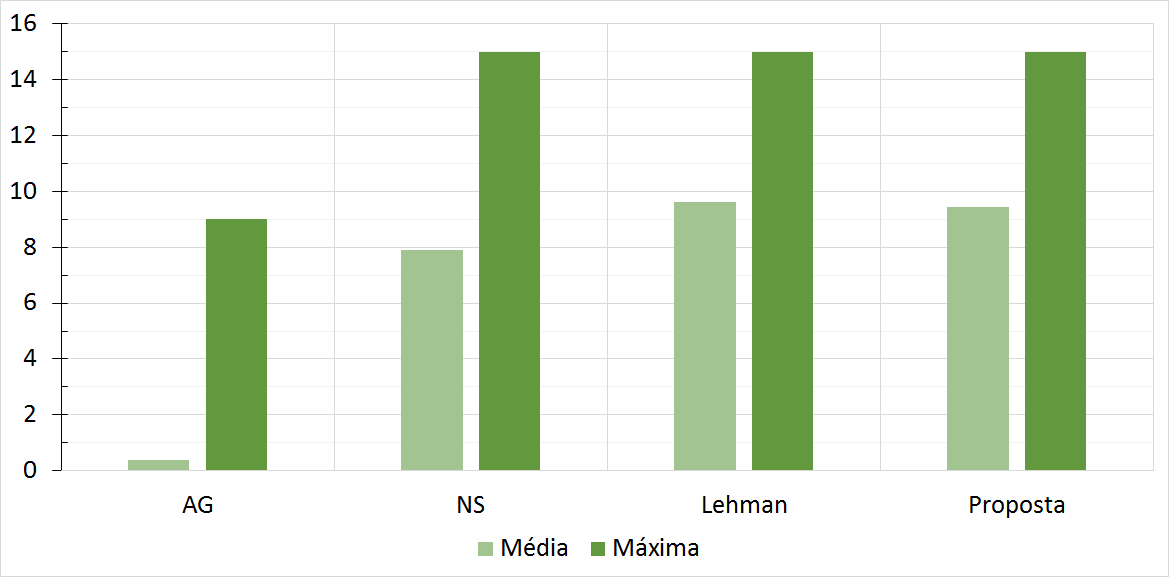
\includegraphics[width=1\textwidth]{Imagens/test_local_comp.png}
		\caption{Gráfico dos valores obtidos para Nota Local Média e Máxima.}
		\label{fig:test_local_comp}
	\end{center}
\end{figure}

Com base nos dados apresentados é possível notar uma grande variação nos valores obtidos pela configuração \textbf{AG} em relação às demais configurações. Esta variação é o esperado, uma vez que a configuração \textbf{AG}, não possui nenhum mecanismo para incentivo à diversidade, gerando assim uma população final com indivíduos muito semelhantes resultando em uma Nota Local baixa; em contrapartida, as demais configurações tem como base a NS, que incentiva a diversidade de seus indivíduos e coopera com a obtenção de maiores valores de Nota Local. Também causa disso, em diversas execuções, a maior nota obtida pela configuração \textbf{AG} não foi capaz de atingir a Nota Local máxima possível (15), enquanto nas demais configurações a nota máxima possível foi obtida ao final de todas as execuções.

Dentre as configurações baseadas na NS, a configuração \textbf{NS} obteve um valor médio um pouco abaixo em relação às configurações \textbf{Lehman} e \textbf{Proposta}, apresentando valores aproximadamente 17\% abaixo dos obtidos por ambas; a variação entre as duas últimas é inferior a dois por cento. A melhoria em relação a nota média obtida por estas configurações finais, se deve ao fato das modificações propostas em \cite{lehman2011evolving} levarem em consideração a Nota Local durante o processo de seleção, incentivando a preservação de indivíduos com boas Notas Locais e melhorando a média geral da população.

\subsection{Quantidade de indivíduos em \texorpdfstring{$C_f$}{Cf}}
\label{metrica_cf_count}

A Tabela \ref{tab:test_cf_count} e gráfico da Figura \ref{fig:test_cf_count} a seguir apresentam a quantidade de indivíduos no conjunto Cf obtidos para todas as configurações ao final de suas execuções.

\begin{table}[htb]
\rowcolors{2}{gray!25}{white}
\centering
\caption{Valores obtidos por cada configuração para a Quantidade de indivíduos em $C_f$.}
\label{tab:test_cf_count}
\resizebox{\textwidth}{!}{%
\begin{tabular}{l|l|l|l|l}
\rowcolor{gray!50}
\hline
\multicolumn{1}{c|}{\textbf{Métrica}} & \multicolumn{1}{c|}{\textbf{Algoritmo Genético}} & \multicolumn{1}{c|}{\textbf{Busca Inovativa}} & \multicolumn{1}{c|}{\textbf{Lehman}} & \multicolumn{1}{c}{\textbf{Proposta}} \\ \hline
Quantidade de indivíduos em $C_f$ & 0.4762 & 12.2500 & 22.6000 & 18.4286 \\ \hline
\end{tabular}%
}
\end{table}

\begin{figure}[htb]
	\begin{center}
		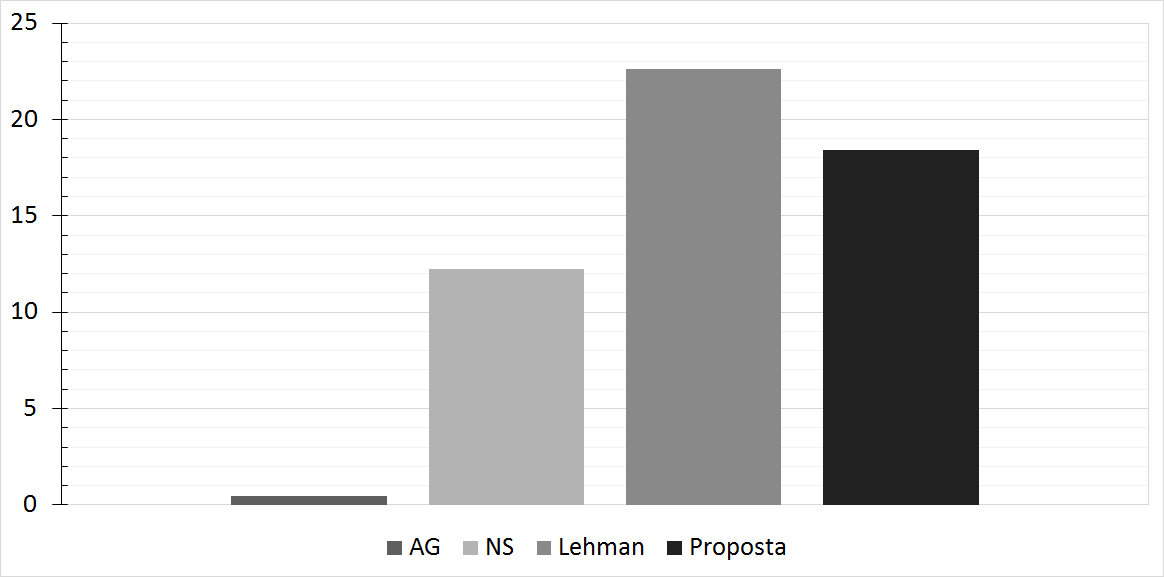
\includegraphics[width=1\textwidth]{Imagens/test_cf_count.png}
		\caption{Gráfico da quantidade de indivíduos em $C_f$.}
		\label{fig:test_cf_count}
	\end{center}
\end{figure}

Assim como para a Nota Loca, e pelos mesmos motivos, há uma grande variação entre os valores obtidos pela configuração \textbf{AG} e as demais. Para esta configuração, em diversas execuções a Nota Local máxima possível (15) não foi atingida, resultando em um conjunto $C_f$ vazio; além disso, quando tal nota foi atingida, o mesmo foi realizado por somente alguns indivíduos, contribuindo ainda mais para uma média geral baixa.

Todas as configurações restantes obtiveram valores muito superiores à configuração \textbf{AG}; com a configuração \textbf{NS}, que obteve a segunda menor quantidade de indivíduos, tendo um valor 2500\% superior à mesma. A maior quantidade de indivíduos obtida foi obtida pela configuração \textbf{Lehman}, com nota 84,49\% superior à configuração \textbf{NS}, comprovando a alta capacidade de exploração e separação de nichos, dados pelas modificações propostas em \cite{lehman2011evolving}, em comparação com a NS. A configuração \textbf{Proposta} obteve resultados 18,46\% inferiores em relação a configuração \textbf{Lehman}; esta redução se deve ao fato de que a configuração \textbf{Proposta} ignora nichos que não possuam alta capacidade funcional, eliminando alguns indivíduos finais pertencentes à nichos de baixa qualidade.

\subsection{Nota de Avaliação}
\label{metrica_nota_avaliacao}

A Tabela \ref{tab:test_fitness} e o gráfico da Figura \ref{fig:test_fitness} a seguir apresentam os valores Nota de Avaliação Média obtidos para todas as configurações ao final de suas execuções, tanto para a população final $P_f$, quanto para os indivíduos do conjunto $C_f$.

\begin{table}[htb]
\rowcolors{2}{gray!25}{white}
\centering
\caption{Valores obtidos por cada configuração para Nota de Avaliação Média em $P_f$ e $C_f$.}
\label{tab:test_fitness}
\resizebox{\textwidth}{!}{%
\begin{tabular}{l|l|l|l|l}
\rowcolor{gray!50}
\hline
\multicolumn{1}{c|}{\textbf{Métrica}} & \multicolumn{1}{c|}{\textbf{Algoritmo Genético}} & \multicolumn{1}{c|}{\textbf{Busca Inovativa}} & \multicolumn{1}{c|}{\textbf{Lehman}} & \multicolumn{1}{c}{\textbf{Proposta}} \\ \hline
Nota de Avaliação Média - $P_f$ & 243.4019 & 63.0031 & 102.2420 & 133.7679 \\ \hline
Nota de Avaliação Média - $C_f$ & N/A & 100.7976 & 134.1249 & 159.3472 \\ \hline
\end{tabular}%
}
\end{table}

\begin{figure}[htb]
	\begin{center}
		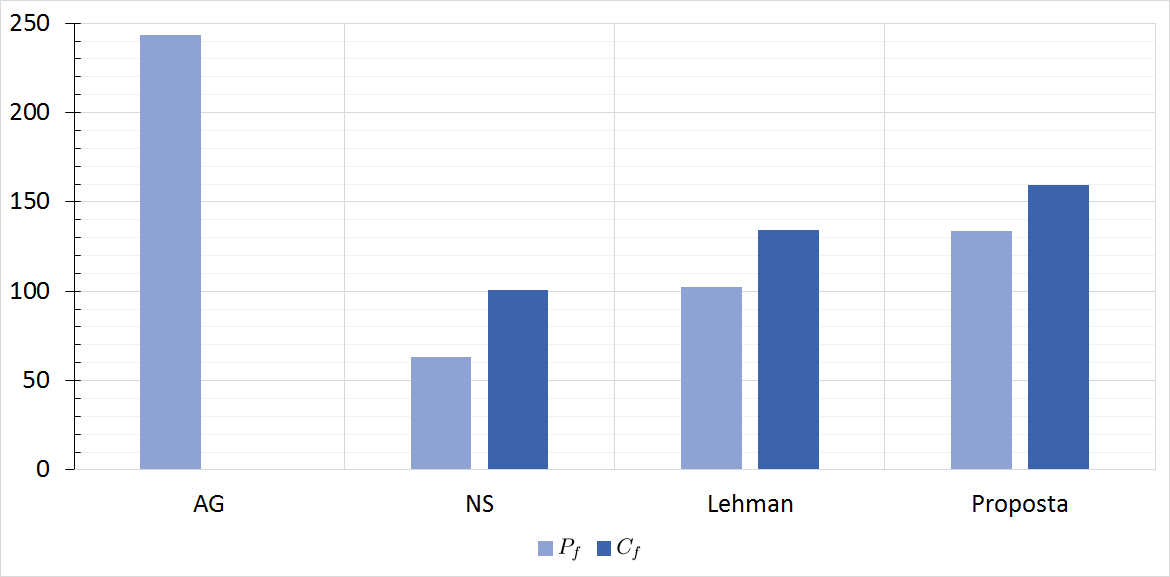
\includegraphics[width=1\textwidth]{Imagens/test_fitness.png}
		\caption{Gráfico das Notas de Avaliação Média obtidas por cada configuração em $P_f$ e $C_f$.}
		\label{fig:test_fitness}
	\end{center}
\end{figure}

Os resultados mostram como a configuração \textbf{AG} é capaz de obter indivíduos extremamente aptos em relação a Função de Avaliação quando comparado com as outras configurações; entretanto, como discutido na seção \ref{metricas}, não é possível definir um conjunto $C_f$ para esta configuração, sendo possível somente a comparação em relação ao valor médio obtido pela população $P_f$.

A configuração \textbf{NS} obteve os piores resultados em relação a Nota de Avaliação, demonstrando a baixa capacidade funcional com o uso da NS sem nenhum mecanismo para recompensar indivíduos funcionais. É importante notar que o uso da NS com outras medidas de comparação, como comportamental por exemplo, é capaz de obter indivíduos mais funcionais \cite{lehman2008exploiting} \cite{lehman2011abandoning}; neste estudo entretanto, utiliza-se uma comparação fenotípica que não está conectada a capacidade funcional do indivíduo, incentivando somente a diversificação específica para o qual foi desenvolvida.

A configuração \textbf{Lehman} obteve resultados superiores aos obtidos pela configuração \textbf{NS} tanto para $P_f$ quanto para $C_f$, sendo 62,28\% e 33,06\% superiores respectivamente. Os resultados obtidos são uma comprovação de que a adição da Função de Avaliação, mesmo que de forma indireta, com a utilização da Competição Local em um MOEA, é capaz de obter indivíduos mais funcionais, embora não seja capaz de atingir a capacidade de um Algoritmo Genético convencional.

A configuração \textbf{Proposta}, mesmo tendo atingido somente 54,96\% do valor médio obtidos para $P_f$ em relação a configuração \textbf{AG}, foi a configuração que obteve melhores resultados dentre as configurações baseadas na NS; em comparação com a configuração \textbf{Lehman}, a qual foi utilizada como base para as modificações propostas, as notas médias para $P_f$ e $C_f$ foram respectivamente 30,89\% e 18,80\% superiores.

\subsection{Dispersão}
\label{metrica_dispersao}

A Tabela \ref{tab:test_dispersion} e o gráfico da Figura \ref{fig:test_dispersion} a seguir apresentam os valores de Dispersão Média obtidos para todas as configurações ao final de suas execuções, tanto para a população final $P_f$, quanto para os indivíduos do conjunto $C_f$.

\begin{table}[htb]
\rowcolors{2}{gray!25}{white}
\centering
\caption{Valores obtidos por cada configuração para Dispersão Média em $P_f$ e $C_f$.}
\label{tab:test_dispersion}
\resizebox{\textwidth}{!}{%
\begin{tabular}{l|l|l|l|l}
\rowcolor{gray!50}
\hline
\multicolumn{1}{c|}{\textbf{Métrica}} & \multicolumn{1}{c|}{\textbf{Algoritmo Genético}} & \multicolumn{1}{c|}{\textbf{Busca Inovativa}} & \multicolumn{1}{c|}{\textbf{Lehman}} & \multicolumn{1}{c}{\textbf{Proposta}} \\ \hline
Dispersão Média - $P_f$ & 35.8831 & 1692.0211 & 1681.9223 & 1550.1303 \\ \hline
Dispersão Média - $C_f$ & N/A & 2044.7265 & 2034.8144 & 1971.9663 \\ \hline
\end{tabular}%
}
\end{table}

\begin{figure}[htb]
	\begin{center}
		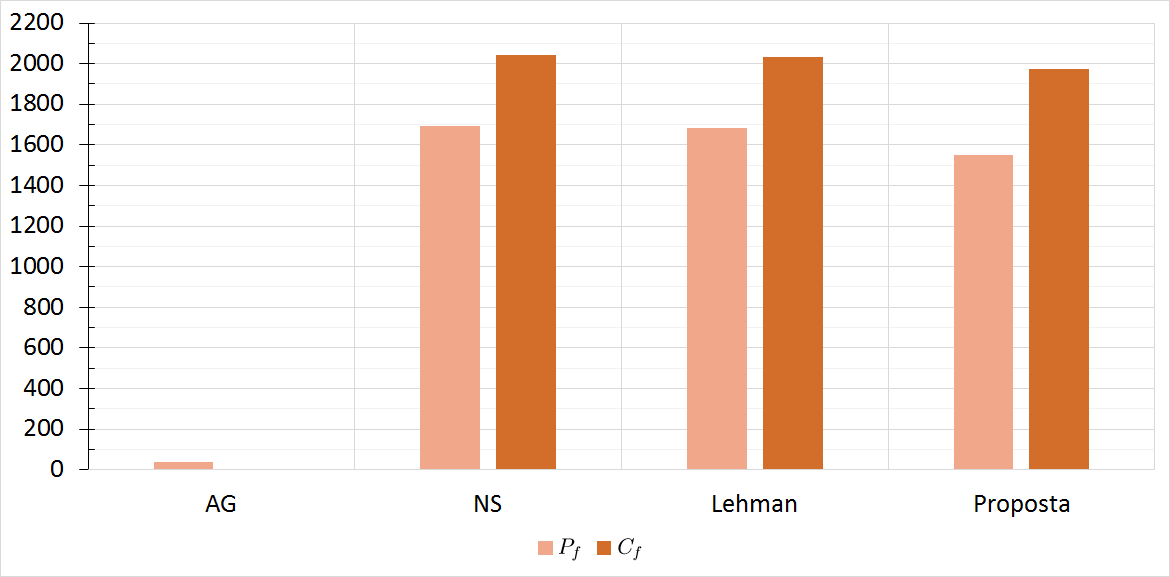
\includegraphics[width=1\textwidth]{Imagens/test_dispersion.png}
		\caption{Gráfico da Dispersão Média obtidas por cada configuração em $P_f$ e $C_f$.}
		\label{fig:test_dispersion}
	\end{center}
\end{figure}

Novamente, através dos resultados obtidos, é possível notar a grande diferença de valores obtidos pela configuração \textbf{AG} em relação às demais configurações. Os valores obtidos para esta configuração comprovam que a população final em Algoritmos Genéticos tende a obter indivíduos extremamente semelhantes, especialmente se comparado com os resultados obtidos pelas configurações que utilizam a NS; essa semelhança justifica tanto a baixa quantidade de indivíduos presentes em $C_f$ quanto os valores obtidos de Nota Local pela configuração. A grande diferença entre os valores demonstra ainda a efetividade da NS em explorar e encontrar indivíduos inovadores.

As configurações \textbf{NS} e \textbf{Lehman} obtiveram os melhores resultados para a métrica de Dispersão tanto para $P_f$ quanto para $C_f$, com uma variação inferior à um por cento entre si. A configuração \textbf{Proposta}, embora tenha obtido a pior nota para a métrica de dispersão dentre as configurações baseadas na NS, ainda obteve valores somente 7,78\% e 3,51\% inferiores às notas $P_f$ e $C_f$ da configuração \textbf{NS} respectivamente.

\subsection{Resultados Obtidos para \texorpdfstring{$C_f$}{Cf}}
\label{metrica_cf}

Para o objetivo desta pesquisa, de obter soluções diversificadas, somente os indivíduos do conjunto $C_f$ são utilizados como solução final. Não sendo capaz de obter indivíduos para o conjunto $C_f$ de forma sólida, como discutido nas seções \ref{metrica_nota_local} e \ref{metrica_cf_count}, e avaliando o valor de Dispersão média obtido, apresentado na seção \ref{metrica_dispersao}; a configuração \textbf{AG} se mostra incapaz de obter soluções que satisfaçam o objetivo proposto. Com isso, uma comparação entre os valores obtidos somente para o conjunto $C_f$ pelas demais configurações se mostra interessante, sendo possível assim analisar dentre as modificações realizadas, quais as vantagens e desvantagens de cada configuração em relação ao objetivo proposto.

O gráfico da Figura \ref{fig:test_cf_compare} apresenta os valores de Dispersão Média e Nota de Avaliação Média obtidos somente pelas configurações baseadas na NS para o conjunto $C_f$ ao final de suas execuções.

\begin{figure}[htb]
	\begin{center}
		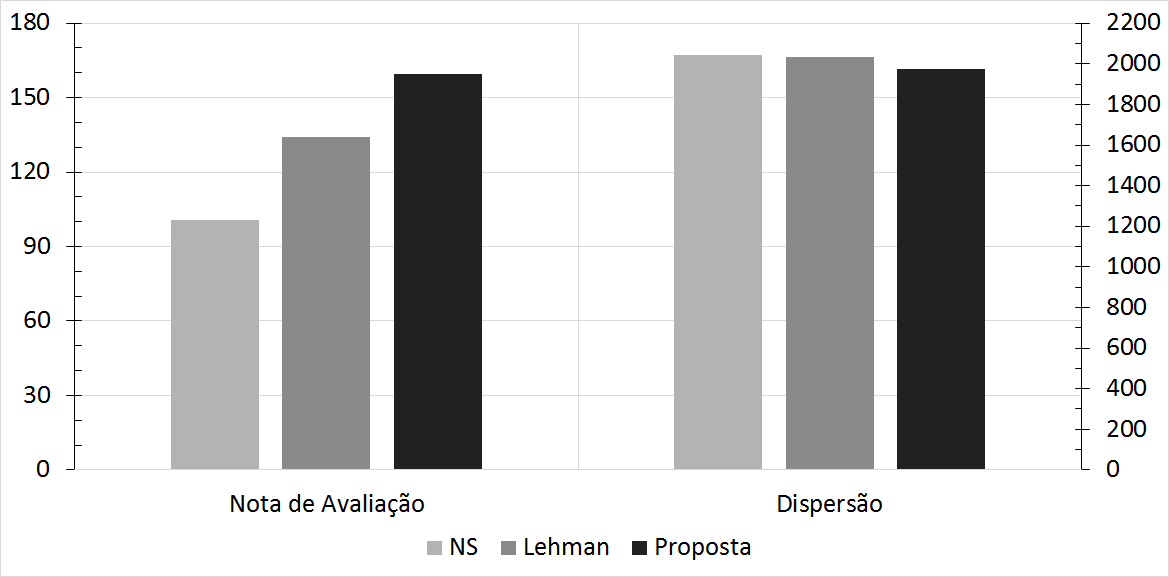
\includegraphics[width=1\textwidth]{Imagens/test_cf_compare.png}
		\caption{Gráfico de Nota de Avaliação Média e Dispersão Média para os conjuntos $C_f$ obtidos em cada uma das configurações baseadas na NS.}
		\label{fig:test_cf_compare}
	\end{center}
\end{figure}

Com base no gráfico apresentado na Figura \ref{fig:test_cf_compare}, pode-se notar um aumento em relação à métrica de Nota de Avaliação pelas modificações propostas em cada configuração. A implementação baseada nas modificações propostas por \textbf{Lehman} obteve um valor 33,06\% superior ao valor obtido pela implementação da \textbf{NS} pura, enquanto a implementação das modificações propostas nesta pesquisa obteve um valor ainda maior, atingindo uma nota 18,80\% superior a configuração \textbf{Lehman} e 58,09\% superior a configuração original \textbf{NS}.

Analisando os valores obtidos para Dispersão, entretanto, é possível notar uma redução de seus números com a introdução das modificações propostas. Enquanto a configuração \textbf{Lehman} obteve somente uma nota de Dispersão 0,48\% inferior à configuração \textbf{NS}, a configuração \textbf{Proposta} obteve uma queda de 3,09\% e 3,56\% em relação às configurações \textbf{NS} e \textbf{Lehman} respectivamente. Embora haja uma queda no valor de Dispersão obtido pela configuração proposta, esta queda é mínima se comparada com o ganho obtido pela introdução da NS em relação ao AG, como visto na seção \ref{metrica_dispersao}; além disso, o ganho em Nota de Avaliação obtido pela configuração \textbf{Proposta} é superior à perda em Dispersão da mesma.

\section{Tempo de Execução}
\label{tempo_de_execucao}

Os testes foram realizados em uma máquina com processador Intel i7-2700k @3.50GHz (8 CPUs) e memória RAM 8192MB. O tempo de execução para cada configuração foi computado de forma total, considerando todas as execuções necessárias para a obtenção da média descrita na seção \ref{resultados_obtidos_jogo_procedural}. Desta forma, o tempo de execução médio de cada configuração é obtido pelo tempo total calculado, dividido pela quantidade de execuções realizadas. Para fins de comparação, o consumo de memória durante as execuções também foi observado. A Tabela \ref{tab:test_time1} apresenta o número de execuções; o tempo total obtido, em segundos; o tempo médio calculado; e o consumo de memória médio para cada configuração.

\begin{table}[htb]
\rowcolors{2}{gray!25}{white}
\centering
\caption{Tempos e consumo de memória em cada execução obtido pelas configurações.}
\label{tab:test_time1}
\resizebox{\textwidth}{!}{%
\begin{tabular}{l|l|l|l|l}
\rowcolor{gray!50}
\hline
\multicolumn{1}{c|}{\textbf{Métrica}} & \multicolumn{1}{c|}{\textbf{Algoritmo Genético}} & \multicolumn{1}{c|}{\textbf{Busca Inovativa}} & \multicolumn{1}{c|}{\textbf{Lehman}} & \multicolumn{1}{c}{\textbf{Proposta}} \\ \hline
Número de Execuções                   & 21                                               & 8                                             & 5                                    & 7                                     \\ \hline
Tempo Total em Segundos               & 875                                              & 1634                                          & 1008                                 & 1401                                  \\ \hline
Tempo Médio de Execução                           & 41.6667                                          & 204.2500                                      & 201.6000                             & 200.1429                              \\ \hline
Consumo Médio de Memória                           & 6.55 MB                                         & 19.80 MB                                     & 19.30 MB                             & 20.25 MB                              \\ \hline
\end{tabular}%
}
\end{table}

Como visto em \cite{cuccu2011novelty}, e verificado pelos valores médios obtidos para tempo de execução e memória, a NS sofre um grande gargalo computacional devido às diversas comparações de distância que devem ser realizadas entre indivíduos da população e do arquivo. Entretanto, se considerarmos a quantidade de indivíduos obtida em média pelas configurações para o conjunto de soluções $C_f$ proposto na seção \ref{dev_conjunto_solucoes}, o tempo computacional por solução se torna aceitável. Uma vez que seriam necessárias várias execuções da configuração \textbf{AG} para obter o mesmo número de resultados para as demais configurações. A diferença de consumo de memória entre as configurações baseadas na NS não é significativo. A Tabela \ref{tab:test_time2} apresenta o tempo médio de execução por solução obtida em cada configuração.

% Please add the following required packages to your document preamble:
% \usepackage{graphicx}
\begin{table}[htb]
\rowcolors{2}{gray!25}{white}
\centering
\caption{Tempo médio de execução por solução obtida em cada configuração.}
\label{tab:test_time2}
\resizebox{\textwidth}{!}{%
\begin{tabular}{l|l|l|l|l}
\rowcolor{gray!50}
\hline
\multicolumn{1}{c|}{\textbf{Métrica}} & \multicolumn{1}{c|}{\textbf{Algoritmo Genético}} & \multicolumn{1}{c|}{\textbf{Busca Inovativa}} & \multicolumn{1}{c|}{\textbf{Lehman}} & \multicolumn{1}{c}{\textbf{Proposta}} \\ \hline
Tempo Médio                           & 41.6667                                          & 204.2500                                      & 201.6000                             & 200.1429                              \\ \hline
Quantidade de indivíduos em $C_f$     & 0.4762                                           & 12.2500                                       & 22.6000                              & 18.4286                               \\ \hline
Tempo Médio por Solução               & 87.4982                                          & 16.6735                                       & 8.9203                               & 10.8604                               \\ \hline
\end{tabular}%
}
\end{table}

Nesta situação, a configuração \textbf{AG} é claramente posta em desvantagem devido à estratégia de soluções proposta, mas, mesmo desconsiderando o conjunto $C_f$, essa tipicamente irá encontrar uma solução por execução. O novo cálculo resultaria em um tempo médio por solução igual a 41,6677 segundos, valor que ainda é inferior aos obtidos por todas as outras configurações.

Os valores revelam ainda, que a configuração \textbf{Proposta} possui um bom desempenho em obter uma quantidade diversificada de soluções, sendo inferior somente à configuração \textbf{Lehman} devido a quantidade de indivíduos em $C_f$ encontrados pela mesma.

\section{Discussão das Análises e Testes}
\label{discussao_analise_e_testes}

Observando-se os resultados obtidos durante os testes é possível verificar a alta capacidade de diversificação introduzida pela NS, com as configurações baseadas na mesma obtendo boas notas nas métrica de Nota Local, Quantidade de indivíduos em $C_f$ e Dispersão. Mesmo a configuração baseada em \textbf{AG} tendo obtido os melhores resultados em relação a Nota de Avaliação, esta não se mostrou capaz de gerar resultados bons o suficiente para o objetivo desta pesquisa, resultando em indivíduos muito semelhantes em sua população final.

Os resultados analisados na seção \ref{metrica_cf} suportam a hipótese de que, no contexto de exploração de indivíduos inovadores, a introdução de um critério mínimo global para restrição da busca, em adição à estratégia de Competição Local apresentada por \cite{lehman2011evolving}, contribui para a melhoria da qualidade funcional dos indivíduos obtidos. Mesmo havendo uma relação de troca em relação à Nota de Avaliação e Dispersão, esta representa um ganho de 18,80 e 58,09 \% para Nota de Avaliação contra uma queda de apenas 3,09 e 3,56 \% para Dispersão em relação as configurações \textbf{NS} e \textbf{Lehman} respectivamente.
